\documentclass[12pt, letterpaper]{article}
\usepackage[utf8]{inputenc}
\usepackage{graphicx}
\graphicspath{{img/}}
\title{Order Types}
\author{Daniel Ulrich
\\
\\
\\
\\
Find another information here:
\\
https://github.com/NakanoMiku13/Research
\\
\\
\\
Find the codes here:
\\
https://github.com/NakanoMiku13/C/blob/Main/QuickSort.c
\\
https://github.com/NakanoMiku13/C/blob/Main/MergeSort.c
\\
}
\date{May 21 2021}
\begin{document}
\maketitle
\newpage
In this file I'll try to explain by the simple mode; \textbf{"What is a order method in programming lenguages?"}
\\ 
In this case when we are talking about order methods we want to make reference to order a number series that are in disorder eg: 7, 4, 3, 1. In this case we need and we want that the series be like this: 1, 3, 4, 7. 
We can have to many options to make this, eg: \textit{Bubble sort, quicksort, mergesort, sort (as the function is in C++)}; but in this case, we are going to explain how it works the \textit{mergesort} and \textit{quick sort} method in C and how to make both.
\\
\\
\title{\textbf{\textit{Mergesort}}}\\
Mergesort is a type of order method that tries to apply the famous \textit{"Divide and conquer"} algorithm, and you'll try to understand this as a normal person, but it could be a little bit complicate if you are not too into this concepts or if you are not used to use it and it is very common; but do not worry, I'll try to explain this as the simple way as I can.
\\
This algorithm will try to divide in two parts the array, in this case lets use this one: [8,2,1,5,3,4];
in this case we can see that the array is in complete disorder, but lets try to order it using this method; the first step that we need, is to know how long is the array, in this case, we know that his size is 6 items (numbers in this case), and then we proceed to divide the array in two equal parts (if it is possible; if it's not possible, do not worry, we can use unpair parts, eg 7 items, we can divide it in 4 and 3), when we make this, we are going to have this "new" 2 arrays [8,2,1] and [5,3,4], then we need to repeat the process, divide this new two arrays into another small arrays, and now we'll have this arrays [5],[3,4],[8],[2,1]; then, lets divide it again; [5],[3],[4],[8],[2],[1]. Easy right? Now, we have to order it, starting by the left-side and order it in small groups of two, in this case to be clear, we start with this pair of numbers [5] and [3], and ask "Who is the biggest one?" 5 or 3 in this case 5 is bigger than 3, and we swap them, and now we have [3,5],[4],[8],[2],[1]. Perfect, now lets do the same with [4] and [8], "who is the biggest one?", in this case 8 is the biggest one, but we have it in order, well, lets go with the next one because we do not have to move anything here; now we have [3,5],[4,8],[2],[1]; well, lets repeat it again, with [2] and [1], "Who is the biggest one?", in this case we are going to have [1,2], and the final array would look like this [3,5],[4,8],[1,2], and now we need to order it in biggest groups, for example groups of 4 items, and order in pairs like the last process, now we check [3,5],[4,8], and check if the first item is bigger or smaller than the first of the second one, in this case 3 is smaller than 4, so we do not need to move anything, then we have 5 and 4, and 5 is bigger, so we swap them, and then we check the 5 and 8, and in this case we can see that 8 is bigger than 5, so it is right, at the end we are going to have this [3,4,5,8],[1,2]; and repeat the process, compare the first and the first, in this case 3 and 1, in this case 1 is smaller than 3, so we add it to the begining, and lets do the same with 3 and 2, so 3 is bigger than 2 so, we add it infront of 3, and then we have this [1,2,3,4,5,8], we have order the number series with the \textit{mergesort} method.
\\
So lets see a graphic example of \textit{mergesort}.
\\
\\
\\
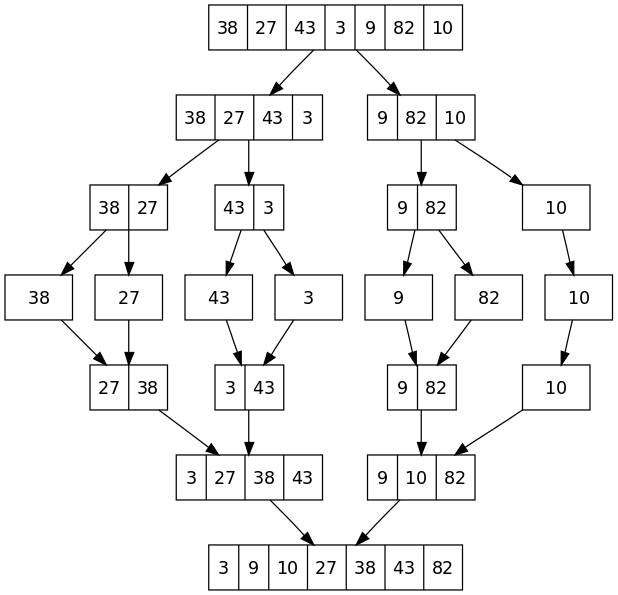
\includegraphics[width=\textwidth]{Merge_sort_algorithm.png}
\\
\\
Now we know how to order item series with \textit{mergesort} method, but lets talk about the advantages and disadvantages about this order method.
\\
\textbf{\textit{Advantages}}
\begin{itemize}
\item Is very useful to sort linked lists
\item Can be modify and optimization as we want
\item Is not a specify formula
\end{itemize}
\textbf{\textit{Disadvantages}}
\begin{itemize}
\item Is slower than other process or algorihtms
\item Requires more memory for the temporary array
\item It could require to repeat too much times some process
\end{itemize}
Now that we know how to this awsome and funny method, lets talk about the second one, that is called, \textit{Quicksort}.
\\
\\
\title{\textbf{\textit{Quicksort}}}\\
So lets talk a little bit about \textit{quicksort}. \textit{Quicksort} is an algorihtm that order the items with the "same" process as \textit{mergesort}, that we need to \textit{"Divide and conquer"}, but in this case we need to choose something that we are going to call "Pivot", in this case the "pivot" could be any number or item in the series (array in this case), eg: we have the same number series as the las example [8,2,1,5,3,4], but lets set a "Pivot", our "Pivot" could be the [4], and now start the process; first of all we need to select the "pivot" when we have the "pivot" we need to divide the rest of the series into two parts, those greater than the "pivot" and those less than the "pivot", in this case we will have this [2,1,3],[4],[8,5], and after this we need to repeat the process with this "new" 2 arrays, we need to select a "pivot" in those numbers less than 4, in this case, it's going to be the number 3, and divide it in those greater and those less, and we will have [2,1],[3], and repeat the process, lets choose a "pivot" and we will have [2],[1], and we order it in base of our "pivot" (I have choose the number 1), and now we have [1],[2],[3],[4],[8,5]; now we repeat the process with the numbers those are great than the 4 and select a "pivot" [5],[8] (I choose the number 5 as "pivot"), and we have finished the \textit{quicksort} process, Why? Because we have this ordered array [1,2,3,4,5,8], and thats all.
\\
Now lets see a new a graphic sample of \textit{quicksort} process.
\\
\\
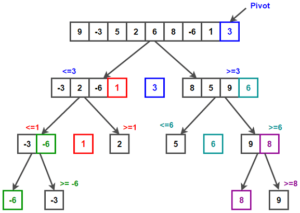
\includegraphics[width=\textwidth]{quicksort-300x213.png}
\\
Now, lets talk about the disadvantages and advantages of the \textit{quicksort} process.
\\
\textbf{\textit{Advantages}}
\begin{itemize}
\item Use less memory than other process
\item In most of the cases the complexity is N log N ops
\item Really short inside process
\end{itemize}
\textbf{\textit{Disadvantages}}
\begin{itemize}
\item In the worst case the complexity is ${N^2}$ ops
\item If we do not make a good implementation, could go unnoticed and cause a really bad performance in the program
\item Is possible that you'll lose the relative order with identical items
\end{itemize}
\newpage
\textbf{References}
\begin{itemize}
\item Alvarez, A. A. (2017, October 7). Ventajas y desventajas de quicksort. QuickSort. $https://quicksortweb.wordpress.com/2017/10/07/ventajas-desventajas-y-aplicaciones/$
\item Fernandez, G. (2019, June 18). Algoritmos de ordenación: Quicksort en Javascript. Leated Code Medium. $https://latteandcode.medium.com/algoritmos-de-ordenaci_C3_B3n-quicksort-en-javascript-f064db39e6ad$
\item GeekForGeek. (2021, May 18). Merge Sort. GeeksForGeeks. $https://www.geeksforgeeks.org/merge-sort/$
\end{itemize}
\end{document}